% !TeX root = ../presentacion.tex


\subsection{Método de elemento finito}

\begin{frame}{Problema de valores propios de Maxwell}{Formulación fuerte y débil del problema de esparcimiento de luz en un volumen $\Omega$}
\small
\begin{alertblock}{\textbf{Formulación fuerte$^1$:} Ecuación diferencial}
				\begin{align*}
					 \nabla \times \qty[\mu^{-1} \nabla \times \vb{E}] - \kappa^2 \vb{E} = \vb{0},
        \qquad
        \text{donde}
        \qquad
        \kappa^2 = (i\omega\sigma +\omega^2 \varepsilon)
    \end{align*}
        \begin{itemize}%[<+->]
         \item  Condiciones de frontera de Dirichlet (D) y de Neumann (N)\vspace*{-.5em}	
    \begin{align*}
    \vu{n}\times \vb{E}(\vb{r})\eval_{\partial \Omega} = \vb{E}_\text{D}
        \qquad\qquad
    \mu^{-1} \nabla \times \vb{E} \times \vu{n} \eval_{\partial \Omega} =  \vb{E}_\text{N}
					\end{align*}
			\end{itemize}
		\end{alertblock}
	
	\begin{alertblock}{\textbf{Formulación  débil$^{1,2}$:} Ecuación integral con el uso de la función de prueba $\boldsymbol{\eta}(\vb{r})$}
        \begin{itemize}%[<+->]
         \item Simplificación mediante integración por partes y teorema de Gauss
					\begin{align*}
					    \int_\Omega \left\{\qty(\mu^{-1}\nabla\times\vb{E})\cdot \qty(\nabla\times\boldsymbol{\eta}) -  \kappa^2  \cdot   \vb{E} \cdot \boldsymbol{\eta} \right\} \dd{\Omega} & - \oint_{\partial\Omega} \qty(\boldsymbol{\eta}\times \vb{E}_\text{N})  \cdot\vu{n}\dd{(\partial\Omega)} = 0
    \end{align*}
    \item Condiciones de frontera \vspace*{-.5em} $$\vu{n}\times \vb{E}(\vb{r})\eval_{\partial \Omega} = \vb{E}_\text{D}.$$
			\end{itemize}
		\end{alertblock}
	
	\noindent\rule{.25\textwidth}{0.4pt}\\    
   \fontsize{4}{5} \selectfont
	$^1$ \fullcite{dhatt_finite_2012}\\
	$^2$ \fullcite{jin_theory_2010}  

\end{frame}

\begin{frame}{Aproximación de elemento finito y método de Galerkin}%
				{Conceptos fundamentales}

   \begin{center}
   
   		$$\text{Sistema de ecuaciones diferenciales en  $\Omega$:}\qquad\mathcal{L}[u(\vb{r})] - {f}_\Omega= {0} \quad	\Longleftrightarrow \quad \int_\Omega \{\mathcal{L}[u(\vb{r})] - {f}_\Omega\}\psi(\vb{r})\dd{\Omega} = 0$$
   
  	\begin{tikzpicture}[node distance=1em and 1em,font=\small]
        \path (0,0) node [flowbox] (fem) {\fbtitle{Elemento finito$^{1-4}$ $\Omega_k$}\vphantom{yÖ}
	    \nodepart{two}
         \begin{minipage}{.28\textwidth} \begin{itemize}
			\item Geometría $$   \bigcup_{k=1}^M \Omega_k = \Omega
        \qquad
    \bigcap_{k=1}^M \Omega_k = \emptyset$$
			\item Espacio de funciones polinomiales $$\{\phi_{i_k}\}_{i_k\leq N_k}$$
			\item Funcional lineal $$\mathcal{F}_{\ell_k}[\phi_{i_k}] = \delta_{{\ell_k}{i_k}}$$
         \end{itemize}\end{minipage}
        };
        
	\node[flowbox,left=of fem] (nodal) {
        \fbtitle{Aproximación nodal$^{1,2}$}\vphantom{yÖ}
    \nodepart{two}
        \begin{minipage}{.28\textwidth}\begin{itemize}
			\item Combinación lineal: $$u(\vb{r}) \approx \sum_i^N u_i \phi_i(\vb{r})$$
			\item Funciones de interpolación : $$\{\phi_{i}\}_{i\leq N}$$
			\item Nodos con valores exactos: $$u_i = u(\vb{r}_i),\;\; \vb{r}_i\in\Omega$$
         \end{itemize}\end{minipage}
    };
    
    	\node[flowbox,right=of fem] (nodal) {
        \fbtitle{Método de Galerkin$^{4}$}\vphantom{yÖ}
    \nodepart{two}
        \begin{minipage}{.30\textwidth}\begin{itemize}
			\item Formulación débil del problema en $\Omega_k$
			\item Funciones de prueba: $$\{\psi_{i_k}\}_{i_k\leq N_k} = \{\phi_{i_k}\}_{i_k\leq N_k}$$
			\item Sistema de ecuaciones algebráicas: $$\mathbb{A} \vb{u} = \vb{f}$$
			donde $A_{i_k j_k} = \int \phi_{i_k}(\vb{r}) \mathcal{L}[\phi_{j_k}(\vb{r})]\dd{\Omega}$, $
				 u_{i_k} = u(\vb{r}_{i_k}) $ y $ f_{j_k} = \int f_{\Omega_k} \phi_{j_k}(\vb{r}) \dd{\Omega}$.
         \end{itemize}\end{minipage}
    };

    \end{tikzpicture}
    \end{center}

	\noindent\rule{.25\textwidth}{0.4pt}\\    
   \fontsize{4}{5} \selectfont
	$^1$ \fullcite{dhatt_finite_2012}\\
	$^2$ \fullcite{larson_finite_2013}\\
	$^3$ \fullcite{jin_theory_2010}\\
	$^4$ \fullcite{fletcher_computational_1984}
	
  

\end{frame}


\begin{frame}{Implementación numérica del problema de esparcimiento de luz}{Familia de elementos finitos de Nédélec$^{1,2}$}

\begin{columns}
\column{.5\textwidth}
 \begin{center}
   
  	\begin{tikzpicture}[node distance=1em and 1em,font=\footnotesize]
        \path (0,0) node [flowbox] (fem) {\fbtitle{Aproximación nodal}\vphantom{yÖ}
	    \nodepart{two}
         \begin{minipage}{.28\textwidth} \begin{align*}
{\vb{E}}(\vb{r}) \approx \sum_{i_k} e_{i_k} \boldsymbol{\eta}_{i_k}(\vb{r})
        \qquad
    e_{i} = \vu{t}_{i_k}\cdot \vb{E}(\vb{r}\in E_{i_k})
\end{align*}\end{minipage}
        };
       
    	\node[flowbox,below=of fem] (nodal) {
        \fbtitle{Método de Galerkin}\vphantom{yÖ}
    \nodepart{two}
        \begin{minipage}{.8\textwidth} $$\mathbb{A} \vb{e} = \vb{0}$$
        \begin{align*}
    A_{ij}  = &    \int_{\Omega_k} \left\{\qty(\mu^{-1}\nabla\times\boldsymbol{\eta}_i)\cdot\qty(\nabla\times\boldsymbol{\eta}_j)
    			-  \kappa^2  \cdot   \boldsymbol{\eta}_i \cdot \boldsymbol{\eta}_j \right\} \dd{\Omega_k} +\\
    		& - \oint_{\partial\Omega} \qty(\boldsymbol{\eta}_j\times \vb{E}_\text{N}) \cdot\vu{n}\dd{(\partial\Omega)}
\end{align*}\end{minipage}
    };
    
    \node[flowbox,below=of nodal]  {
        \fbtitle{Funcional de Nédélec de menor orden}\vphantom{yÖ}
    \nodepart{two}
        \begin{minipage}{.85\textwidth}
        $$ \mathcal{F}^{N}_{i_k}[\boldsymbol{\eta}_{\ell_k}(\boldsymbol{\xi})] = \frac{1}{\abs{E_{i_k}}}\qty(\int_{E_{i_k}} \vu{t}_{i_k}\cdot\boldsymbol{\eta}_{\ell_k}(\boldsymbol{\xi})   \dd{(\partial\Omega_k)} )^{1/2}  $$\end{minipage}
    };

    \end{tikzpicture}
    \end{center}   

\column{.5\textwidth}\centering
Para geometrías triangulares:
$$\boldsymbol{\eta}_{i_k} = \abs{E_{i_k}} \qty(\phi_{j_k}\nabla\phi_{\ell_k} - \phi_{\ell_k}\nabla\phi_{j_k} )$$
$$\mathcal{F}^{L}_{\ell_k}[\phi_{j_k}(\boldsymbol{\xi})] = \phi_{j_k}(\boldsymbol{\xi}_{\ell_k})$$
\begin{figure}
    \fontsize{4}{5} \selectfont
    \def\svgwidth{1\textwidth}
    \includeinkscape{FEM-Theory/P1-Example-Nedelec}
\end{figure}


\end{columns}
    \vspace*{-.0em}\fontsize{4}{5} \selectfont
   \noindent\rule{.25\textwidth}{0.4pt}\\
	$^1$ \fullcite{jin_theory_2010}\\
	$^2$ \fullcite{larson_finite_2013}
\end{frame}

\subsection{Condiciones de frontera abiertas}
\begin{frame}{Condiciones de frontera abiertas}{Simulando medios infinitos }

\begin{description}
	\item[\textbf{Condición de radiación de Sommerfeld$^1$:}] Comportamiento en el campo lejano 
	$$
    \lim_{r\to\infty} \qty(\vu{e}_r\times\vb{E} - \sqrt{\frac{\mu}{\varepsilon}} \vb{H}) = \lim_{r\to \infty} r\qty(\nabla\times \vb{E} - i k \vu{e}_r\times\vb{E}) = 0  $$
	\item[\textbf{\textit{Perfect Matching Layer$^2$:}}] Película ($\Omega_\text{PML}$) sin impedancia y absorbente basada en su geometría:
	\begin{align*}
	        \left. \mqty{\varepsilon_{{}_\Omega}=\varepsilon_{{}_\text{PML}} ,
                                                &\mu_{{}_\Omega}=\mu_{{}_\text{PML}}
                                                \\
                                                \\
                                            s^{(\Omega)}_x  = s^\text{(PML)}_x,
                                            &  s^{(\Omega)}_y  = s^\text{(PML)}_y} \right\}
                    \qquad\implies \qquad
           r_\text{s} = r_\text{p} = 0 .
\end{align*}	
\end{description} 
\begin{center}
   
  	\begin{tikzpicture}[node distance=1em and 1em,font=\small]
        \path (0,0) node [flowbox] (fem) {\fbtitle{Método de Galerkin$^3$}\vphantom{yÖ}
	    \nodepart{two}
         \begin{minipage}{.28\textwidth}	\begin{align*}
	 \mathbb{A}\vb{e} = \vb{0} \qquad &\text{con}\qquad \text{ $\mathbb{A}$ y $\vb{e}$ definidas anteriormente,}\\
         \mathbb{\Lambda} = \text{diag}\qty(s_z, s_z ,s_z^{-1}),      \qquad&\text{con}\qquad     s_z= 1 \text{ en } \Omega \text{ y } \Im[s_z] < 0 \text{ en } \Omega_\text{PML}, \\
         \qty(\mu^{-1}\nabla\times\boldsymbol{\eta}_i)\cdot\qty(\nabla\times\boldsymbol{\eta}_j)   \qquad&\to\qquad   \qty(\mathbb{\Lambda}^{-1}\mu^{-1}\nabla\times\boldsymbol{\eta}_i)\cdot  \qty(\nabla\times\boldsymbol{\eta}_j),\\
         \boldsymbol{\eta}_i \cdot \boldsymbol{\eta}_j  \qquad&\to\qquad  \boldsymbol{\eta}_i \cdot \mathbb{\Lambda} \boldsymbol{\eta}_j,
	\end{align*}\end{minipage}
        };
       
    
    \node[right=of fem]  {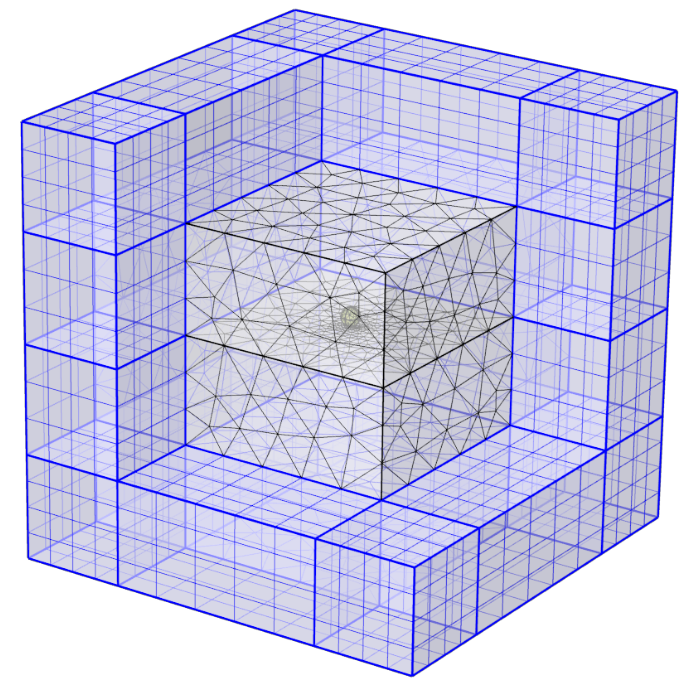
\includegraphics[scale=.2]{Geometries/sist}    };

    \end{tikzpicture}
    \end{center}   
    \vspace*{-1em}\fontsize{4}{5} \selectfont
   \noindent\rule{.25\textwidth}{0.4pt}\\
$^1$ \fullcite{silver_microwave_1984}\\
	$^2$ \fullcite{chew_complex_1997}\\
	$^3$ \fullcite{jin_theory_2010}\\

\end{frame}

































